\documentclass[main.tex]{subfiles}
%\graphicspath{{\subfix{../images/}}}
\begin{document}
\begin{enumerate}[label=\textbf{\alph*)}]
    \item O gráficos ficaram bem parecidos com o da primeira questão para $\alpha = 1$, o que era de se esperar, já que o movimento da questão 1 se dá à pequenos ângulos, pode-se aproxima-lo por um oscilador harmônico.
    Como exemplo, temos o gráfico de $\theta \times t$ e da energias do sistema.
    \begin{center}
        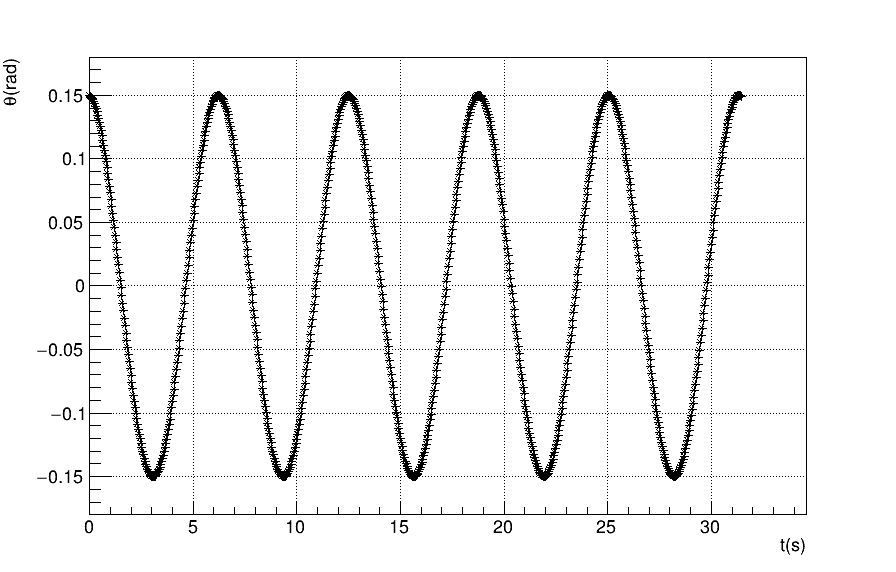
\includegraphics[scale=0.15]{../q3/plots/theta_t_ec.png}
        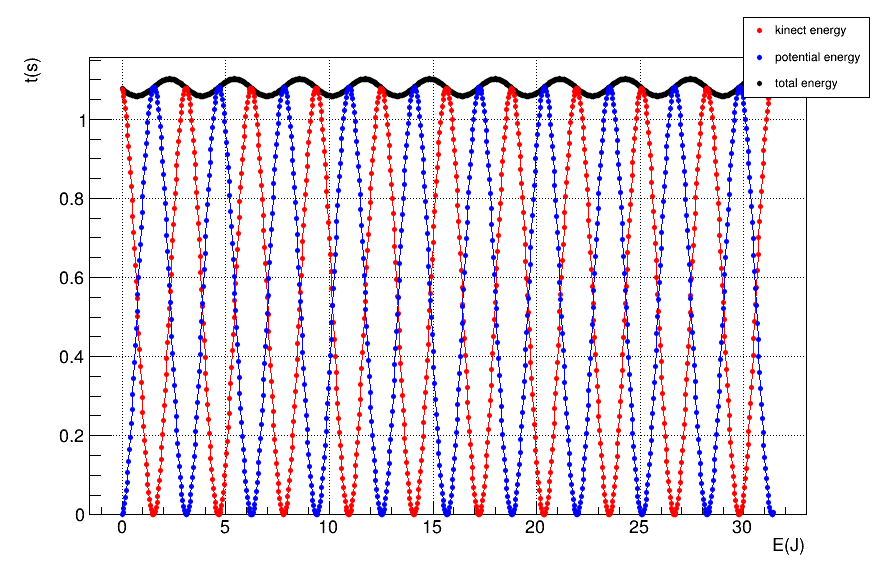
\includegraphics[scale=0.15]{../q3/plots/Energies_t_ec.png}
        \captionof{figure}{Gráfico de $\theta \times t$ (à esquerda) e Energia em função do tempo (à direita) para o oscilador harmônico simples com $\alpha = 1$.}
    \end{center}
    Nesse caso, o $k$ tem dimensão de $\frac{1}{[s]^2}$.
    \item     
    \begin{center}
        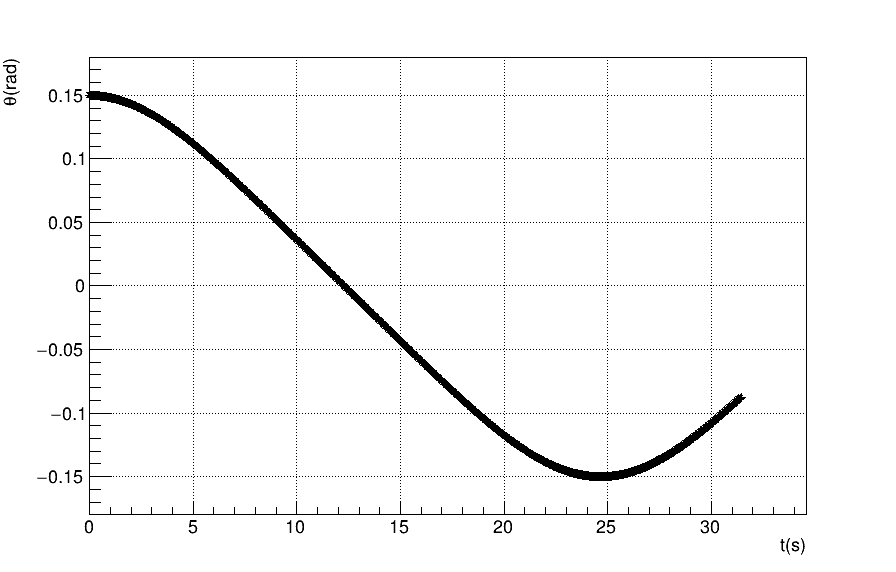
\includegraphics[scale=0.15]{../q3/alpha3/theta0.2/plots/theta_t_ec.png}
        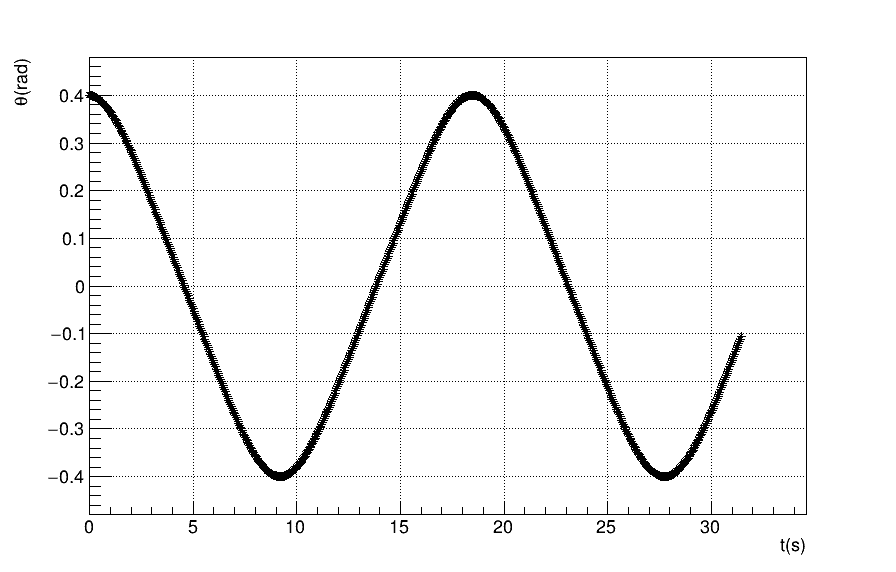
\includegraphics[scale=0.15]{../q3/alpha3/theta0.4/plots/theta_t_ec.png}
        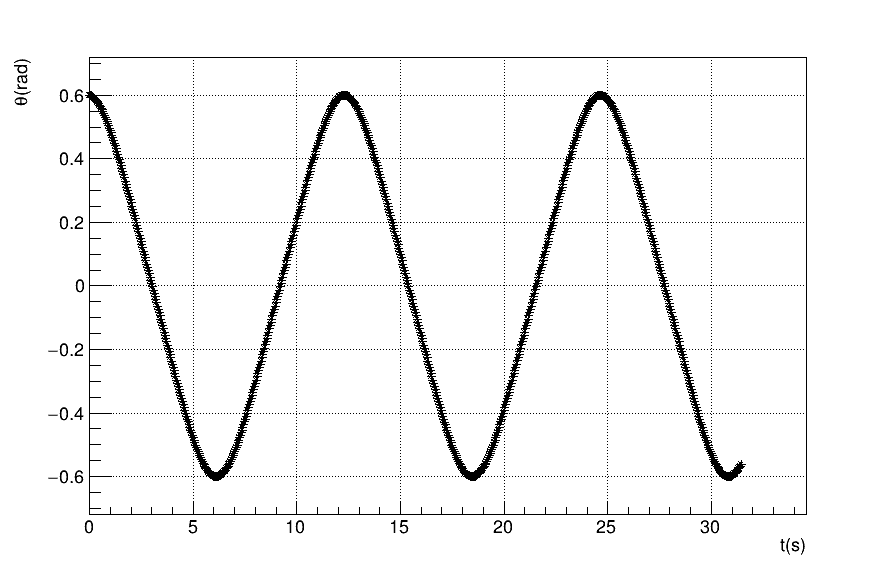
\includegraphics[scale=0.15]{../q3/alpha3/theta0.6/plots/theta_t_ec.png}
        % \captionof{figure}{Gráfico de $\theta \times t$ (à esquerda) e Energia em função do tempo (à direita) para o oscilador harmônico simples com $\alpha = 1$.}
    \end{center}
    \begin{center}
        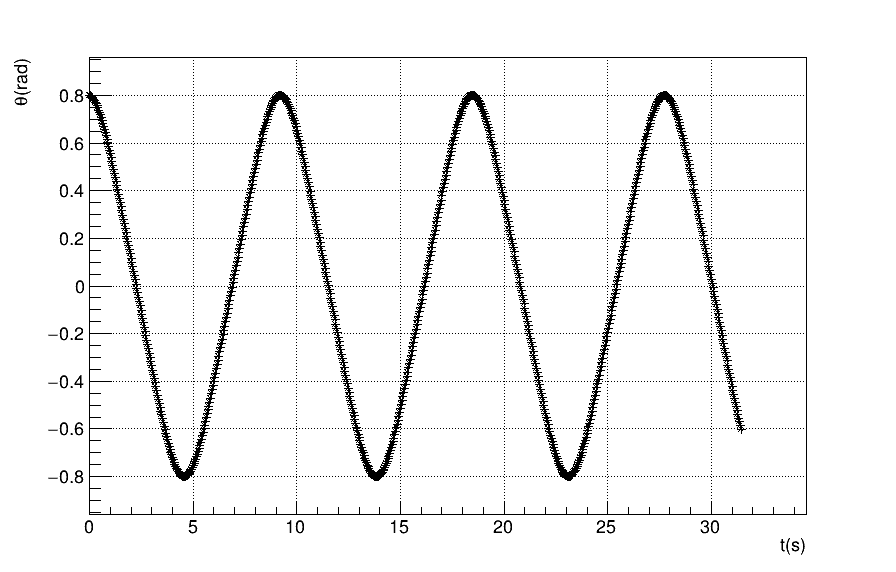
\includegraphics[scale=0.15]{../q3/alpha3/theta0.8/plots/theta_t_ec.png}
        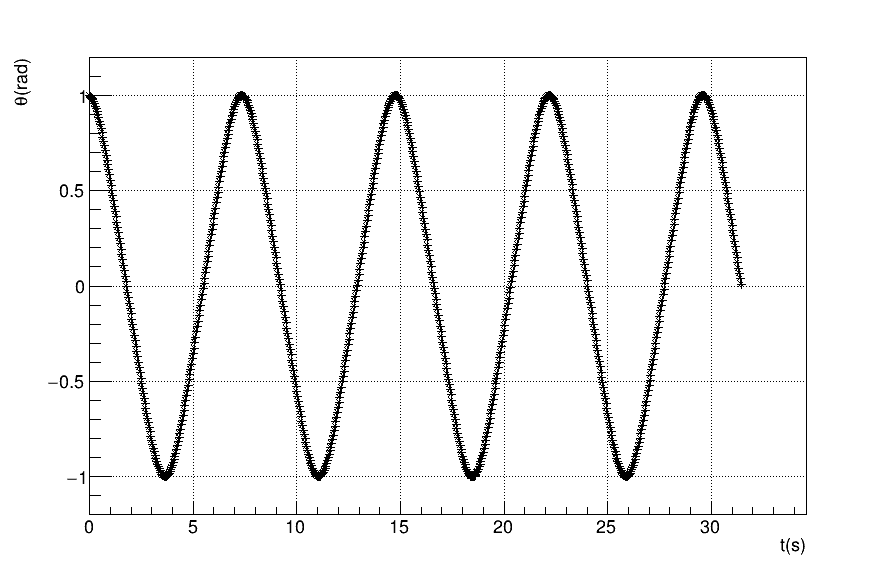
\includegraphics[scale=0.15]{../q3/alpha3/theta1/plots/theta_t_ec.png}
        % \captionof{figure}{Gráfico de $\theta \times t$ (à esquerda) e Energia em função do tempo (à direita) para o oscilador harmônico simples com $\alpha = 1$.}
    \end{center}
\end{enumerate}

\end{document}